
\chapter{Background}

\textit{Parts of this chapter have been published as J.\ Varennes, and A.\ Mugler, ``Sense and sensitivity: physical limits to multicellular sensing, migration, and drug response,'' Molecular pharmaceutics 13.7 (2016): 2224-2232.}
\vspace{5mm}

Cells can sense very small concentration gradients \cite{shields2007autologous} and may also act collectively
\cite{cheung2013collective, friedl2012classifying, aceto2014circulating, puliafito2015three}.
We review the physical limits to sensory precision by discussing the basic theory of concentration and gradient sensing by cells and multicellular collectives. This theory places physical limits to sensory precision due to extrinsic noise caused by the diffusing chemical.

\section{Single-cell concentration sensing}

Theoretical limits to the precision of concentration sensing were first introduced by Berg and Purcell 40 years ago \cite{berg1977physics}. Berg and Purcell began their study by considering an idealized cell that acts as a perfect counting instrument. The cell is assumed to be spherical and molecules can freely diffuse in and out of it (Fig.\ \ref{fig:ch1_2}A). The concentration of these molecules is uniform in space, and the cell derives all its information about the concentration by counting each molecule inside its spherical body. The expected count is
$\bar{n} = \bar{c}V$ where $\bar{c}$
is the mean concentration and $V$ is the cell volume. However, since molecules arrive and leave via diffusion, there will be fluctuations around this expected value. Diffusion is a Poisson process, meaning that the variance in this count $\sigma_n^2$ equals the mean $\bar{n}$. Therefore the relative error in the cell's concentration estimate is
$\sigma^2_c/\bar{c}^2 = \sigma_n^2/\bar{n}^2 = 1/(\bar{c} V)$.

\begin{figure}[ht]
    \centering
        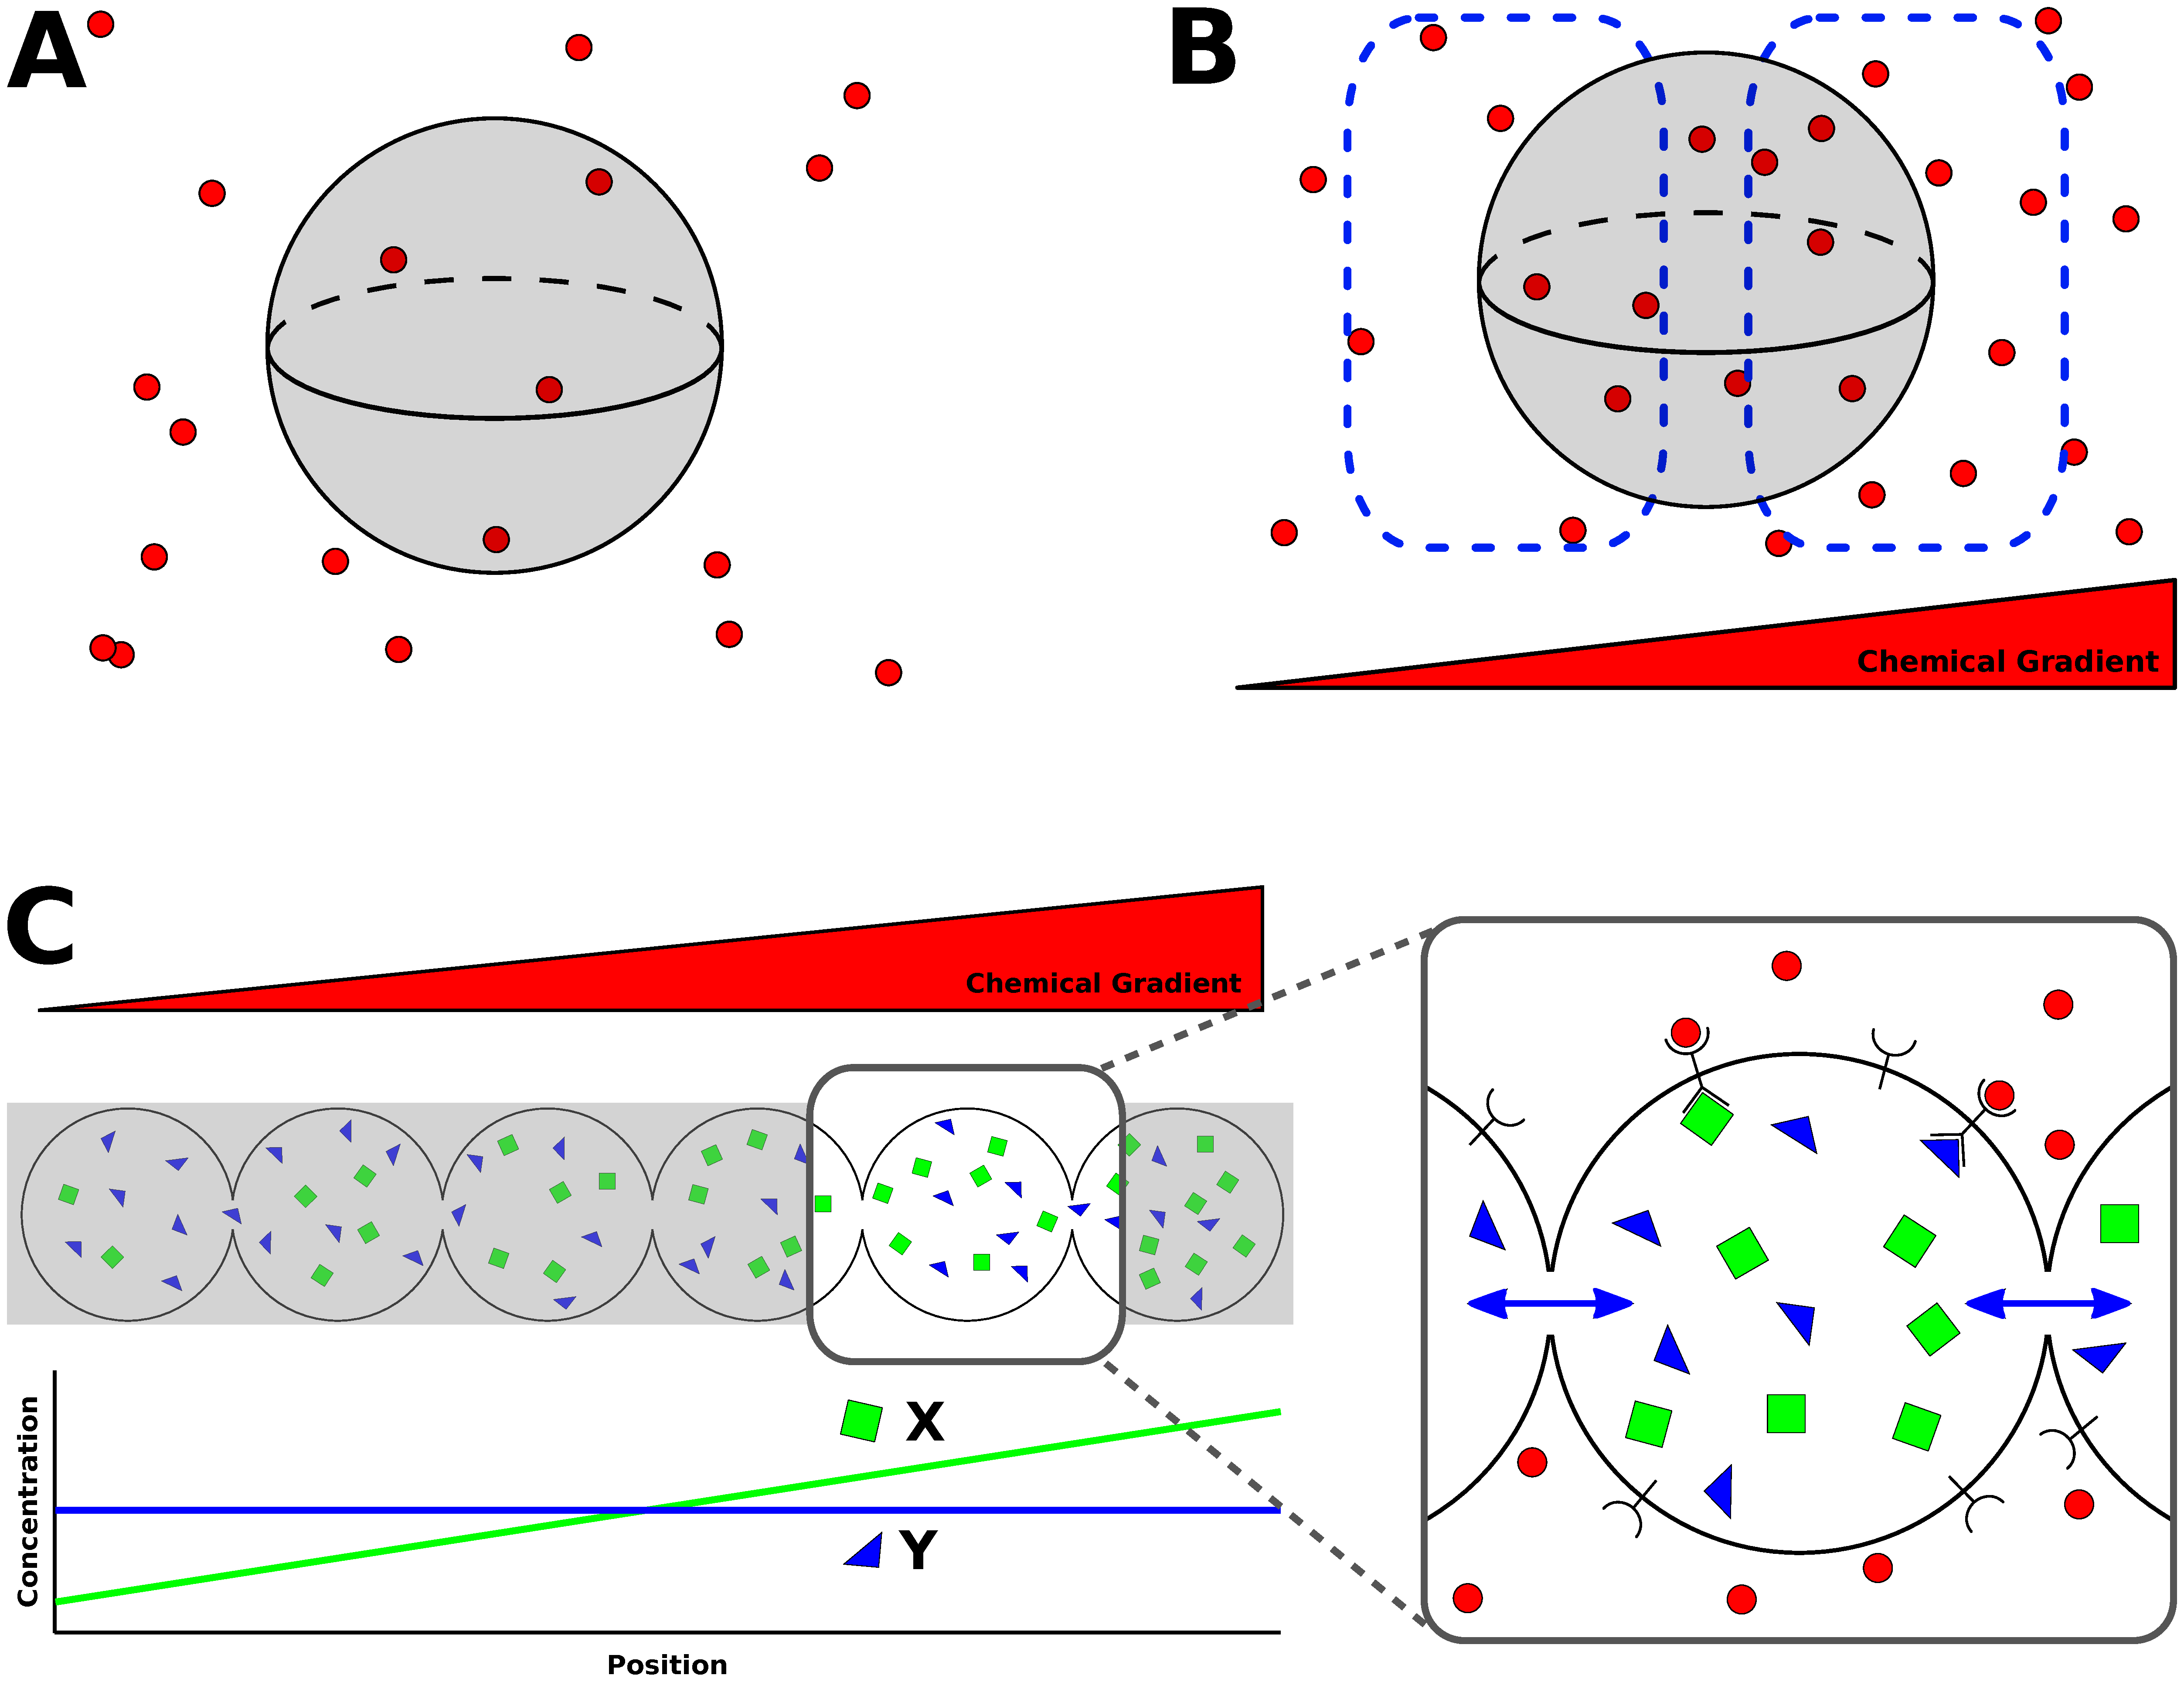
\includegraphics[width=0.8\textwidth]{../fig/ch1_fig2.pdf}
    \caption{Deriving the limits to concentration and gradient sensing.
    (A) An idealized cell as a permeable sphere that counts molecules inside its volume.
    (B) A cell counts molecules in two compartments in order to estimate a concentration gradient.
    (C) The local excitation--global inhibition (LEGI) model of multicellular gradient sensing. $Y$ molecules diffuse between neighboring cells, whereas $X$ molecules do not. The difference between $X$ and $Y$ counts in a given cell reports the extent to which that cell's concentration measurements are above the average.}
    \label{fig:ch1_2}
\end{figure}

The cell can improve upon the relative error in its concentration estimate by time-averaging over multiple measurements. However, consecutive measurements are only statistically independent if they are separated by a sufficient amount of time such that the molecules inside the cell volume are refreshed. The amount of time required is characterized by the diffusion time, $\tau \sim V^{2/3}/D \sim a^2/D$, where $D$ is the diffusion constant and $a$ is the cell diameter. In a time period $T$ the cell makes $\nu = T/\tau$ independent measurements, and the variance is reduced by the factor $1/\nu$. This gives the long-standing lower limit
\begin{equation} \label{eq:ch1_c1}
\frac{ \sigma_c^2 }{\bar{c}^2} = \frac{ \sigma_n^2}{\bar{n}^2} \sim \frac{1}{a\bar{c}DT}
\end{equation}
for the cell's relative error in estimating a uniform concentration.
The relative error decreases with $a$ and $\bar{c}$, since the molecule count is larger, and also with $D$ and $T$, since more independent measurements can be made. Berg and Purcell derived this limit more rigorously \cite{berg1977physics}, and the problem has been revisited more recently to account for binding kinetics, spatiotemporal correlations, and spatial confinement \cite{bialek2005physical, kaizu2014berg, bicknell2015limits}.
In all cases a term of the form in Eq.\ \ref{eq:ch1_c1} emerges as the fundamental limit for three-dimensional diffusion.

Does cell sensory performance reach this limit in real biological contexts? Berg and Purcell themselves addressed this question using the \textit{Escheria coli} bacterium \cite{berg1977physics}. Motility of \textit{E.\ coli} has two distinct phases: the run phase in which a cell swims in a fixed direction, and the tumble phase in which the cell erratically rotates in order to begin a new run in a different direction. The bacterium biases its motion by continually measuring the chemoattractant concentration, and extending the time of runs for which the change in concentration is positive \cite{berg1977physics,dahlquist1976studies}. The change in concentration $\Delta \bar{c} = Tv\bar{g}$
over a run time $T$ depends on the concentration gradient
$\bar{g} = \partial \bar{c} / \partial x$
and the bacterium's velocity $v$. Berg and Purcell argued that for a change in concentration to be detectable, it must be larger than the measurement uncertainty,
$\Delta \bar{c} > \sigma_c $.
Together with Eq.\ \ref{eq:ch1_c1}, this places a lower limit on the run time,
$T > [ \bar{c}/(aDv^2\bar{g}^2)]^{1/3}$.
Using typical values \cite{berg1977physics} for the sensory threshold of \textit{E.\ coli} of
$\bar{c} = 1$ mM, $\partial \bar{c} / \partial x = 1$ mM/cm, $a=1$ $\mu$m, $v=15$ $\mu$m/s, and $D=10^{-5}$ cm$^2$/s, we find $T > 0.1$ s.
Actual run times are on the order of $1$ s. Thus we see that \textit{E.\ coli} chemotaxis is consistent with this physical bound. The fact that actual run times are not too much longer than the minimum indicates that the sensory machinery of \textit{E.\ coli} operates near the optimal precision of a perfect counting device. If \textit{E.\ coli} were to use much shorter run times, there would be no way to acquire sufficient statistics, and chemotaxis would be physically impossible.

\section{Single-cell gradient sensing}

Unlike \textit{E.\ coli} bacterium, larger cells do not need to swim in order to detect temporal changes in concentration. Larger cells, like amoeba, epithelial cells, neutrophils, and neurons, sense gradients by comparing concentration measurements between spatially separate compartments along the cell body \cite{jilkine2011comparison}. These compartments are typically receptors or groups of receptors on the cell surface, but in a simple model we may treat these compartments as idealized counting volumes as we did for concentration sensing. The difference in counts between two such compartments provides the cell with an estimate of the gradient (Fig.\ \ref{fig:ch1_2}B). Following the same procedure as for concentration sensing we can derive the relative error in gradient sensing.

Consider two compartments of linear size $s$ on either side of a cell with diameter $a$ (Fig.\ \ref{fig:ch1_2}B). Given that the compartments are aligned with the gradient $\bar{g}$ of a linear concentration profile, then the mean concentrations at each compartment are $\bar{c}_1$ and
$\bar{c}_2 = \bar{c}_1 + a\bar{g}$.
The mean molecule counts in the two compartments are roughly $\bar{n}_1 = \bar{c}_1s^3$ and $\bar{n}_2 = \bar{c}_2s^3$, and the difference is $\Delta\bar{n} = \bar{n}_2 - \bar{n}_1 = a\bar{g}s^3$. The variance in this difference is
$\sigma_{\Delta n}^2 = \sigma_{n_1}^2 + \sigma_{n_2}^2 \sim \bar{n}_1^2/(s\bar{c}_1DT) + \bar{n}_2^2/(s\bar{c}_2DT)$,
where the first step assumes the two compartments are independent, and the second step uses Eq.\ \ref{eq:ch1_c1} for the variance in each compartment's measurement. For shallow gradients, where the limits on sensing are generally reached, $a\bar{g} \ll \bar{c}_1$, and so $\bar{c_1} \approx \bar{c_2} \approx \bar{c}$, where $\bar{c}$ is the mean concentration at the center of the cell. Thus
$\sigma_{\Delta n}^2 \sim 2(\bar{c}s^3)^2/(s\bar{c}DT)$,
and the relative error in the cell's estimate of the gradient is then
\begin{equation} \label{eq:ch1_g1}
    \frac{\sigma_g^2}{\bar{g}^2} = \frac{ \sigma_{\Delta n}^2}{ \Delta \bar{n}^2} \sim \frac{\bar{c}}{s(a\bar{g})^2DT},
\end{equation}
where the factor of $2$ is neglected in this simple scaling estimate. Similar to Eq.\ \ref{eq:ch1_c1}, the relative error in gradient sensing decreases with $s$, since larger compartments allow for larger molecule counts. The relative error also decreases with $D$ and $T$, since they increase the number of independent measurements. Additionally, the relative error decreases with $a\bar{g}$, since the concentrations measured by the two compartments are more different from each other. However, we see that unlike Eq.\ \ref{eq:ch1_c1}, the relative error increases with the background concentration $\bar{c}$. The cell is measuring a concentration difference, not the concentration itself, and it is more difficult to accurately measure a small difference on a larger background than on a smaller background \cite{ellison2016cell}.
Eq.\ \ref{eq:ch1_g1} has been derived more rigorously in other studies \cite{endres2009accuracy}, and the problem has been extended to describe different receptor configurations and geometries
\cite{endres2008accuracy,endres2009accuracy,hu2010physical}.
In all these cases, the relative error has a term similar to Eq.\ \ref{eq:ch1_g1}, with the lengthscale $s$ dictated by the particular sensory mechanism and geometry. The optimal mechanism would result in an effective compartment size that is roughly half of the cell volume, in which case $s\sim a$.

Experiments on the amoeba \textit{Dictyostelium discoideum} have tested the limits to gradient sensing \cite{van2007biased}. \textit{Dictyostelium} cells exhibit biased movement when exposed to gradients of cyclic adenosine monophosphate as small as $\bar{g} = 10$ nM/mm, on top of a background concentration of $\bar{c} = 7$ nM. Bias is typically quantified in terms of the chemotactic index (CI), which is the cosine of the angle between the gradient direction and the direction of a cell's actual motion. By relating the error in gradient sensing (a term of the form in Eq.\ \ref{eq:ch1_g1} with $s = a$) to the error in this angle, Endres and Wingreen \cite{endres2008accuracy} obtained an expression for the optimal CI, which they then fit to the experimental data with one free parameter, the integration time $T$.
The inferred value of $T = 3.2$ s serves as the physical lower bound on the response time required to perform chemotaxis. Actual response times of \textit{Dictyostelium} cells, as measured by the time from the addition of a chemoattractant to the peak activity of an observable signaling pathway associated with cell motility \cite{postma2003uniform, parent2004making}, are about $5-10$ s. Taken together, these results imply that \textit{Dictyostelium} operates remarkably close to the physical limit to sensory precision set by the physics of molecule counting.


\section{Multicellular gradient sensing}

Next, we turn our attention to multicellular gradient sensing. In many biological processes, such as metastatic invasion \cite{cheung2013collective, friedl2012classifying}, cells behave in a collective manner. Collectives of cells sense shallower gradients than single cells, both in terms of percent concentration changes and absolute molecule numbers (Table \ref{sense_table}). For example, neuron collectives respond to gradients equivalent to a difference of less than one molecule across an individual neuron's growth cone \cite{rosoff2004new}. It is likely that this benefit in sensory precision found in collectives also translates to better chemotaxis for collectives. This may be a reason why collective invasion is sometimes observed during metastasis.

From Eq.\ \ref{eq:ch1_g1} we see that a multicellular collective has lower sensory error because it is larger than a single cell. The cell collective spans a larger portion of the concentration profile, leading to a larger difference between the concentration measurements on either end, and a lower relative error. In terms of Eq.\ \ref{eq:ch1_g1}, if we consider that cells on the ends act as the molecule-counting compartments, $s \to a$, and that the entire collective acts as the detector, $a \to Na$, where $N$ is the number of cells in the gradient direction, then we have \cite{mugler2016limits}
\begin{equation} \label{eq:ch1_g2}
    \frac{\sigma_g^2}{\bar{g}^2} \sim \frac{\bar{c}}{a(Na\bar{g})^2DT}.
\end{equation}
As expected, the relative error goes down with the size $Na$ of the multicellular collective.

It is important to note that in formulating Eq.\ \ref{eq:ch1_g2} we have overlooked any loss of precision caused by communicating sensory information across the collective. The larger the group of cells, the more difficult it will be for cells on either end to communicate measurement information. Eq.\ \ref{eq:ch1_g2} does not account for this, and assumes that any error induced by the communication process is negligible. In fact, Eq.\ \ref{eq:ch1_g2} states that the relative error decreases with increased collective size. For a single cell it may be a reasonable approximation to assume that compartments quickly and reliably communicate information across the cell body, but for a multicellular collective, the communication process should deteriorate as the collective grows in size. This process introduces additional noise to the collective's gradient sensing abilities. Therefore, it is imperative when considering collective sensing to properly account for the effects of communication.

Recent studies have explored the physical limits to collective gradient sensing for different communication mechanisms and collective geometries
\cite{ellison2016cell, mugler2016limits, fancher2016fundamental}.
In two of the studies \cite{ellison2016cell, mugler2016limits} communication was modeled using a multicellular version of the local excitation--global inhibition (LEGI) paradigm \cite{levchenko2002models}, in which each cell produces a ``local'' and a ``global'' molecular species in response to the chemical in the environment. The global species is exchanged between cells to provide the communication, whereas the local species remains within the cell it was produced (Fig.\ \ref{fig:ch1_2}C). The difference between local and global molecule numbers in a cell provides it with information about the chemical gradient. A positive difference informs the cell that its measured concentration (represented by the local species) is above the spatial average among its neighbors, and therefore that the cell is located up the gradient, not down.
The relative error of gradient sensing for the LEGI model was shown \cite{mugler2016limits} to be limited from below by
\begin{equation} \label{eq:ch1_g3}
    \frac{\sigma_g^2}{\bar{g}^2} \sim \frac{\bar{c}}{a(n_0a\bar{g})^2DT},
\end{equation}
where $n_0^2$ is the ratio of the global species' cell-to-cell exchange rate to its degradation rate. When communication is accounted for the error is bounded by $n_0a$, whereas in Eq.\ \ref{eq:ch1_g2} the error decreases indefinitely with size $Na$. The communication strength defines an effective number of cells $n_0$ over which information can be reliably conveyed, and a collective that grows beyond this size no longer improves its sensory precision.

The communication-limited relative error prediction was tested experimentally in epithelial cell collectives \cite{ellison2016cell}. Mouse mammary epithelial cells were grown in organotypic culture and subjected to very shallow gradients of epidermal growth factor (Table \ref{sense_table}). While single epithelial cells did not respond to the gradient, the multicellular collectives exhibited a biased cell-branching response. Critical to communication-limited prediction, the response of large collectives was no more biased than that of small collectives, supporting the idea that communication sets an effective collective size. From experiments the effective collective size was inferred to be $n_0 \approx 3.5$ cells, which is consistent with the collective sizes found in nature (the ``end buds'' of growing mammary ducts) \cite{lu2008genetic}.
Communication between cells is mediated by gap junctions between cells, and experiments show that when gab junctions are blocked, the biased response in collectives vanished \cite{ellison2016cell}. This demonstrates that collective response is critically dependent on cell-to-cell communication. Taken together, these results indicate that communication is a necessary but imperfect component of collective gradient sensing. The results also speak to the power of simple physical theory to quantitatively explain collective cellular capabilities. Many epithelial cancers are known to invade collectively \cite{cheung2013collective}, and these theoretical predictions may also describe the sensory behavior of metastatic cell collectives.


\section{Relative changes vs.\ absolute molecule numbers}

The precision of gradient sensing is often reported in terms of percent concentration change across a cell body. For example, both amoeba \cite{van2007biased} and tumor cells \cite{shields2007autologous} are sensitive to a roughly $1\%$ change in concentration across the cell body. However, this method of reporting sensitivity may be misleading. Experiments imply very different sensory thresholds for these cells in terms of absolute molecule numbers, as we will now see.

The key is that it takes two numbers to specify the conditions for gradient sensing: the mean gradient $\bar{g}$ and the mean background concentration $\bar{c}$. For the amoeba \textit{Dictyostelium}, these numbers are $\bar{g} = 10$ nM/mm and $\bar{c} = 7$ nM at the sensory threshold \cite{van2007biased}. Given a typical cell size of $a = 10$ $\mu$m, these values imply a mean percent concentration change of $\bar{p} = a\bar{g}/\bar{c} = 1.4\%$ (Table \ref{sense_table}). However, we may also compute from these values the mean molecule number difference
$\Delta\bar{n} = a\bar{g}s^3$
from one side of the cell to the other, within the effective compartments of size $s$. Taking $s\sim a$ gives the maximal molecule number difference of $\Delta\bar{n} = a^4\bar{g} = 60$
for \textit{Dictyostelium} (Table \ref{sense_table}). Together $\bar{p}$ and $\Delta\bar{n}$ specify the sensing conditions as completely as $\bar{g}$ and $\bar{c}$ do.

\begin{table*}[t]
\begin{center}
\begin{tabular}{ |l|c|c|c|c| }
\hline
\multirow{2}{*}{ }
& \multicolumn{2}{ |c| }{Single Cell} & \multicolumn{2}{ |c| }{Multicellular} \\ \cline{2-5}
 & \textit{Dictyostelium}
 & Breast
 & Neurons \cite{rosoff2004new}
 & Mammary \\
& (Amoeba) \cite{van2007biased}
& Cancer \cite{shields2007autologous}
& & Epithelia \cite{ellison2016cell} \\
\hline
Cell Length & 10 $\mu$m & 20 $\mu$m & 10 $\mu$m & 10 $\mu$m \\
Scale, $a$  & & & & \\ \hline
Background & 7 nM & 1100 nM & 1 nM & 2.5 nM \\
Concentration, $\bar{c}$  & & & & \\ \hline
Concentration & 10 nM/mm & 550 nM/mm & $0.1$ nM/mm & $0.5$ nM/mm \\
Gradient, $\bar{g}$ & & & & \\ \hline
Percent Concentration & 1.4\% & 1.0\% & 0.1\% & 0.2\% \\
Difference, $\bar{p} = \bar{g}a/\bar{c}$ &  &  &  &  \\ \hline
Molecule Number & 60 & 53,000 & 0.6 & 3 \\
Difference, $\Delta\bar{n} = \bar{g}a^4$ & & & & \\ \hline
\end{tabular}
\caption{Gradient sensory thresholds for single cells and multicellular collectives. Note that experiments can provide equal percent concentration differences but unequal molecule number differences across a cell body, as seen for amoeba and breast cancer cells. We see that multicellular groups can detect smaller gradients than single cells by all measures.}
\label{sense_table}
\end{center}
\end{table*}

Experiments \cite{shields2007autologous} have shown that breast cancer tumor cells exhibit a chemotactic response in a gradient $\bar{g} = 550$ nM/mm of the cytokine CCL21, on top of a background concentration of $\bar{c} = 1100$ nM. Given a typical cell size of $a = 20$ $\mu$m, this corresponds to a percent difference of
$\bar{p} = a\bar{g}/\bar{c} = 1\%$,
similar to \textit{Dictyostelium}. Yet, this also corresponds to a maximal molecule number difference of
$\Delta\bar{n} = a^4\bar{g} = 53,$$000$,
which is much higher than that of \textit{Dictyostelium} (Table \ref{sense_table}). Even though the sensitivities are similar in terms of percent change, they are very different in terms of absolute molecule number.

Lower molecule numbers correspond to higher relative error. We can see this explicitly by writing Eq.\ \ref{eq:ch1_g1} in terms of the percent change $\bar{p} = a\bar{g}/\bar{c}$. Defining $\epsilon = \sigma_g/\bar{g}$ and taking $s \sim a$, we have
$\epsilon \sim 1/\sqrt{\bar{p}^2a\bar{c}DT}$.
Accounting for the fact that tumor cells (TC) have roughly twice the diameter as \textit{Dictyostelium} cells (DC), this expression implies that the sensitivities of the two cell types over the same integration time $T$ to chemoattractants with the same diffusion constant $D$ satisfy
$\epsilon_{\rm DC}/\epsilon_{\rm TC} = \sqrt{2\bar{c}_{\rm TC}/\bar{c}_{\rm DC}} \approx 18$.
We see that because the \textit{Dictyostelium} experiments were performed at lower background concentration, corresponding to lower absolute molecule numbers, the relative error in gradient sensing is $18$ times that of the tumor cells, despite the fact that both cell types are responsive to $1\%$ concentration gradients. Therefore, it is important to take note of the background concentration when studying the precision of gradient sensing. These data imply that \textit{Dictyostelium} cells can sense noisier gradients than tumor cells. However, \textit{Dictyostelium} cells have been studied more extensively than tumor cells as exemplars of gradient detection. It remains an interesting open question what is the minimum gradient that tumor cells can detect, not only in terms of percent concentration change, but also in terms of absolute molecule number differences.


\section{Models of cell migration and chemotaxis}

Next we review models of migration since chemotaxis involves both sensing and movement. From a physical modeling perspective, describing collective cell dynamics is an interesting problem, because often rich and unexpected behavior can emerge from a few simple interaction rules between cells \cite{vicsek1995novel,coburn2013tactile}.
Even in the absence of sensing, simple models have successfully explained observed collective behaviors such as cell streaming, cell sorting, cell sheet migration, wound healing, and cell aggregation \cite{kabla2012collective,szabo2010collective,basan2013alignment,janulevicius2015short}.
Although cell migration has been studied on a single-cell basis \cite{shao2010computational}, oftentimes unique collective behavior emerges from studying multicellular models.


\subsection{Mechanisms of collective migration}

We will focus specifically on collective dynamics in which sensory cues play a key role in the emergent behavior. Chemoattractants in the environment are detected by cells and causing the polarization of a single cell or cell collective via one of a variety of mechanisms \cite{jilkine2011comparison}, and the resulting migratory dynamics are directed.
Mechanisms of collective migration can largely be divided into three categories. First, cells may exhibit individual sensing and individual migration (Fig.\ \ref{fig:ch1_3}A). Here, each cell can perform gradient sensing and migration individually, although the precision may be low. When many such cells are placed in a group, the group migration can be enhanced and focused by local interactions between the cells. Even if each individual cell has low sensory and migratory precision, the precision of the group as a whole is high due to the interactions. This mechanism is often termed ``many wrongs,'' and it is successful at explaining how group migratory behavior emerges from individual agents that act independently \cite{coburn2013tactile,simons2004many}.
For example, a recent study demonstrated that single-cell chemotaxis can be improved through collisions between cells which align cell polarization in the gradient direction \cite{coburn2013tactile}. Collisions act to average over the errors in individual cells' noisy measurements, thereby decoupling group behavior from single-cell properties. We develop a simple model of individual-based chemotaxis in conjuction with chemotaxis experiments in Ch.\ 2, and in Ch.\ 3 we analyze the effects of extrinsic noise on collectives of individually chemotaxing cells.


\begin{figure}[ht]
    \centering
        \includegraphics[width=0.8\textwidth]{../fig/ch1_fig3.pdf}
    \caption{Mechanisms of collective migration: (A) individual sensing and migration (the ``many wrongs'' mechanism), (B) individual sensing but collective migration (emergent chemotaxis), and (C) collective sensing and migration. Implementations of collective migration: (D) in force-based models, dynamics evolve from stochastic forces acting on each cell; (E) in energy-based models, dynamics evolve via energy minimization with thermal noise. E shows the cellular Potts model framework, in which cells are collections of lattice sites, and cell-cell (dashed blue) and cell-environment (dashed yellow) contacts contribute to the energy of the system.}
\label{fig:ch1_3}
\end{figure}


Second, cells may exhibit individual sensing but collective migration (Fig.\ \ref{fig:ch1_3}B). In this mechanism, each individual cell senses its own local environment, and tight mechanical interactions result in the emergent directed motion of the entire group. This mechanism is applicable to the collective migration of connected clusters of cells. For example, a model of this type was recently developed by Camley et al.\ to describe behavior seen in clusters of neural crest cells and other cell types \cite{camley2016emergent}. In this model, cells are tightly connected but are polarized away from neighboring cells due to contact inhibition of locomotion (CIL), the physical phenomenon of cells ceasing motion in the direction of cell-cell contact \cite{mayor2010keeping}. Individual cells sense a local chemoattractant concentration and attempt to migrate away from the group with a strength proportional to this concentration.
However, the mechanical coupling keeps them together. In the presence of a concentration gradient, the imbalance in their migration strengths results in net directed motion (Fig.\ \ref{fig:ch1_3}B). Notably, this mechanism results in directed motion of a cluster even though individual cells cannot execute directed motion alone, since without other cells, there is no CIL to bias the motion. In Ch.\ 3 we develop an analytical model to study the effects of extrinsic noise on cell collectives analogous to that illustrated in Fig.\ \ref{fig:ch1_3}B.

Third, cells may exhibit collective sensing and collective migration (Fig.\ \ref{fig:ch1_3}C). As discussed above, multicellular groups exploit cell-to-cell communication to sense gradients collectively, thereby enhancing the precision of sensing. A feature of this collective sensing, e.g.\ via the multicellular LEGI mechanism discussed above \cite{ellison2016cell, mugler2016limits}, is that each cell has information on the extent to which it is up or down the gradient. Through CIL or other contact-mediated interactions, this information can translate directly into cell polarity, leading to more coherent collective migration than in the previous mechanism (Fig.\ \ref{fig:ch1_3}C vs.\ B).
In fact, the multicellular LEGI model was used by Camley et al.\ \cite{camley2016emergent} to explore a model of this type. Adding collective sensing to their model of CIL-dependent migration gave the advantage that the repulsive tension on a cell cluster was adaptive and therefore remained constant as the cluster migrated to regions of higher chemical concentration. In Ch.\ 4, we present a computational model of collective chemotaxis in which the effects noise caused by the environment as well as intercellular communication of explicitly accounted for.

\subsection{Model implementations}

To study the above mechanisms quantitatively and compare predictions with experiments, one must turn to mathematical and computational modeling. Models of cell dynamics range from continuum or semi-continuum descriptions, which describe groups of cells as continuous tissues, to individual-based models, which describe cells as individual interacting entities \cite{shao2010computational,maclaren2015models,camley2017physical}.
Physics-driven individual-based models generally fall into two categories: force-based models and energy-based models.

Force-based models (Fig.\ \ref{fig:ch1_3}D) typically represent cells as centers of mass or as collections of vertices. Cell dynamics evolve from forces acting on individual cells, which can be stochastic, and arise from internal features such as cell polarity, and external features such as mechanical interactions with other cells \cite{maclaren2015models}.
Force-based models are able to reproduce multicellular behavior such as chemotaxis, wound healing, and cell aggregation \cite{camley2016emergent,basan2013alignment,janulevicius2015short}. Parameters are often directly relatable to experimental measurements, and the simplest models are often amenable to exact mathematical analysis \cite{camley2016emergent}.

Energy-based models (Fig.\ \ref{fig:ch1_3}E) allow cell dynamics to emerge from the minimization of a potential energy with thermal noise (the so-called Monte Carlo scheme). A widely used example is the cellular Potts model (CPM) \cite{graner1992simulation, swat2012multi}, in which cells are represented as collections of co-aligned ``spins'' on a lattice (Fig.\ \ref{fig:ch1_3}E). Cells remain contiguous because it is energetically favorable for neighboring spins to be co-aligned. Biophysical features such as cell shape, cell-cell adhesion, and cell protrusions into the environment are modeled by introducing corresponding terms into the global potential energy.
The CPM has been used to describe cell sorting, streaming, and chemotaxis \cite{maree2007cellular} and has successfully reproduced experimental observations of epithelial streaming, cell sorting, and collective migration \cite{kabla2012collective,maree2007cellular,szabo2010collective}.
In energy-based models, the parameters are less directly relatable to experiments; rather, their values can often be set by calibrating emergent features, such as cell diffusion coefficients or average speeds, with experimental measurements \cite{szabo2010collective}.


\section{Summary}

In summary, we have reviewed the physical limits of concentration and gradient sensing, the sensitivity of cells and multicellular collectives, and various modeling techniques for cell migration. Chemotaxis is a process of sensing, polarization and migration. However, how all three components come together remains an open question. Our goal is to investigate how extrinsic noise in chemoattractant concentration detection affects chemotaxis for single cells and multicelluar collectives. In doing so we hope to better understand the limits to chemotactic performance, as well as the role that collective effects have in improving performance.


% Although the physical limits to multicellular sensing are becoming better understood, the physical limits constraining multicellular migration are less clear. This remains an interesting open question, and answering it will require integrating the theories of sensing and communication with the models of collective migration described herein. For tumor cells in particular, an integrated physical theory of sensing and migration would prove immensely useful for identifying the key determinants of invasive capabilities. Identifying these determinants would help pinpoint the ways that these capabilities could be disrupted, using drugs and other therapies, as described next.


% In summary, we took a quantitative look at metastatic invasion as a chemotactic process, which has allowed us to compare metastatic cells to other cell types in terms of their physical capabilities. We have seen that tumor cells can sense very shallow chemoattractant gradients, which may help guide metastatic invasion, but it remains unclear whether tumor cells  operate near fundamental sensing limits, as bacteria and amoeba do. Recognizing that metastatic invasion can be collective, we have reviewed recent results on the physical limits to collective sensing, and we have identified the overarching mechanisms of collective migration. A key insight that emerges is that the chemotactic capabilities of cell collectives rely critically on intercellular interactions such as cell-cell communication.

% Identifying whether the physical theory of sensing reviewed herein can be applied in a predictive manner to cancerous cell-types, and whether gradient sensing plays a dominant role during metastatic invasion is still an active field of research. Moreover, it is important to integrate the theory of sensing with models of collective migration to quantitatively predict the chemotactic performance of multicellular collectives. Controlled experiments of cancer cells are necessary to validate these predictions.
% This may open up the possibility for alternative cancer therapy strategies that target specific intercellular functions such as communication, in addition to typical therapeutic that aim for comprehensive cell death.

% \red{...to assess the viability of alternative therapies that target specific cell functions in order to combat metastatic invasion. Our hope is that the integrated, physics-based perspective presented herein will help generate innovative solutions to the pervasive problem of metastatic disease.}


% Cells gather information about their environment by sensing chemical concentrations and concentration gradients. In fact, cells can do this with remarkable precision. The amoeba \textit{Dictyostelium discoideum} is sensitive to differences on the order of ten molecules between its front and back half \cite{song2006dictyostelium}. It is therefore natural to ask how well cells can sense their environment, and whether the error in the sensing capabilities can be quantified. These questions were first answered by Berg and Purcell almost 40 years ago \cite{berg1977physics}. They considered a simplified model of a cell in order to calculate a lower limit on the relative error in its measurement of a chemical concentration, and they also showed that the sensory machinery of the \textit{Escheria coli} bacterium operates very near this physical bound.
% The question of how well single cells measure chemical concentrations has been revisited to account for binding kinetics, spatiotemporal correlations and spatial confinement
% \cite{bialek2005physical, kaizu2014berg, bicknell2015limits}.
% These studies have helped shape our understanding of how cells sense their environment. However, in nature cells are rarely found alone, and the interactions between nearby cells may alter cells' sensory capabilities.

% In many biological contexts cells act in close proximity to one another so their interactions may not be easily ignored when trying to understand the physical limits to sensing. In fact, these interactions can enhance cell sensitivity to the environment. Using communication, clusters of mammary epithelial cells can detect chemical gradients that single cells cannot \cite{ellison2016cell}, and cultures of neurons have been shown to be sensitive to single molecule differences across an individual neuron's axonal growth cone \cite{rosoff2004new}.
% In studying multicellular sensing of chemical concentrations and gradients it is important to recognize that in order to collect these spatially separated measurements from individual cells the information must be communicated to some common location. Explaining how cells efficiently communicate information has been the topic of recent research. Similar to the limits set by Berg and Purcell, the physical limits to communicated, collective gradient sensing have been derived \cite{mugler2016limits,ellison2016cell} by using a multicellular version of the local excitation-global inhibition (LEGI) communication model \cite{levchenko2002models}, one of the simplest adaptive mechanisms of gradient sensing. With these studies the physical limits of cell sensing have been extended from single cells to multicellular collectives.

% In parallel to studies on collective sensing, much recent work has focused on collective cell behavior, including migration. For example, processes in development, cellular migration, pathogenic response, and cancer progression all involve many cells acting in a coordinated way
% \cite{friedl2010plasticity,
% rasmussen2006quorum, boelens2014exosome, cheung2013collective, vader2014extracellular}.
% Work has been done in studying how these multicellular systems behave from a mechanical perspective. Simple mechanical models have successfully explained observed collective behaviors such as cell streaming, cell sorting, cell sheet migration, wound healing, and cell aggregation \cite{kabla2012collective,szabo2010collective,basan2013alignment,janulevicius2015short}. Though these studies accurately model some form of collective cell migration they fail to include the effects of multicellular sensing in driving the mechanics at play. In many biological systems, cells are capable of communicating with one another, so understanding how these cells translate that information into mechanical action is of prime interest.

% Here we focus our attention on collective cell migration and how cells use multicellular communication to direct their motion. As summarized, much is known regarding multicellular communication and its physical limits as well as how to model the mechanics of collective behavior. The connection between these two fields, however, is missing. The primary goal of this research is to connect the studies of the physical limits of cell communication to those of cellular dynamics in order to gain deeper insight into collective behavior. These two fields can be connected by creating a model which links the collective sensing output to the polarization of migrating cells. Furthermore, by creating numerical simulations of collective sensing and migration we can relate our model to real biological systems.

% One multicellular system of particular interest is that of cancer metastasis. The first step in metastasis is the invasion of tumor cells into the surrounding micro-environment. Invasion is known to occur in a highly organized manner that likely involves communication \cite{cheung2013collective,friedl2012classifying,vader2014extracellular}. Recent work shows that tumor cell invasion is guided by sensory cues to blood vessels and to lymphatics, and that cancer cells can sense their environment with remarkable precision \cite{shields2007autologous}. It is clear that the early stages of metastasis depend on cell sensing and in certain types of cancer, occur in a collective manner. Hence understanding how the limits of multicellular sensing affect collective cell migration can help us better understand how collective tumor cell invasion occurs.

% In conjunction with the development and analysis of a model of collective sensing and migration, work with experimental collaborators will help verify whether the proposed model can indeed reproduce experimental results. In developing any theoretical model it is important to be able to validate or disprove the model through experiments. This will be achieved through our collaboration with Professor Bumsoo Han of Purdue University and his research group, who will observe how breast cancer cells migrate in the presence of a chemoattractant gradient. Developing a theoretical model alongside experiment will enable us to verify its accuracy and also match theoretical parameters with experimental observables in order to extend the model to more biological systems.

% Metastasis is one of the most intensely studied stages of cancer progression because it is the most deadly stage of cancer. The first step of metastasis is invasion, wherein cells break away from the tumor and invade the surrounding tissue. Our understanding of metastatic invasion has benefited tremendously from genetic and biochemical approaches \cite{leber2009molecular, hanahan2000hallmarks, hanahan2011hallmarks}. However, the physical aspects of metastatic invasion are still unclear \cite{hanahan2011hallmarks}. We know that at a fundamental level, metastatic invasion is a physical process. Tumor cells sense and respond to chemical gradients provided by surrounding cells
% \cite{bhowmick2004stromal, condeelis2006macrophages, shields2007autologous, puliafito2015three} or other features of the tumor environment
% \cite{shields2007autologous, polacheck2011interstitial, shieh2011regulation} (Fig.\ \ref{fig:ch1_1}A). Indeed, tumor cells are highly sensitive, able to detect a $1\%$ difference in concentration across the cell length
% \cite{shields2007autologous}. Sensing is ultimately a physical phenomenon. Therefore, can we build a simple physical theory to understand the sensory behavior of tumor cells, and can this physical theory inform treatment options?
%
% Metastatic invasion involves coordinated migration of tumor cells away from the tumor site. In many types of cancer, migration is collective and highly organized, involving the coherent motion of connected groups of cells
% \cite{cheung2013collective, friedl2012classifying, aceto2014circulating, puliafito2015three}
% (Fig.\ \ref{fig:ch1_1}B).
% Collective migration is ultimately a physical phenomenon, since it relies on mechanical coupling and can often be understood as emerging from simple physical interactions at the cell-to-cell level. Can we understand the collective migration of tumor cells with simple physical models?
%
% Here we review recent progress on modeling sensing and migration in cells and cell collectives. We discuss metastatic cells explicitly, and emphasize that physical insights gained from other cellular systems can inform our understanding of metastatic invasion. We focus on simple physical models and order-of-magnitude numerical estimates in order to quantitatively probe the extent of, and the limits to, cell sensory and migratory behavior. Our hope is that a more quantitative understanding of metastatic invasion will inform treatment protocols, and to that end we conclude by discussing drug sensitivity and potential treatment strategies (Fig.\ \ref{fig:ch1_1}C).

% \subsection{Single-cell gradient sensing}
%
% Unlike \textit{E.\ coli}, larger cells like tumor cells do not need to swim to detect gradients. Larger cells, including amoeba, epithelial cells, neutrophils, and neurons, sense gradients by comparing concentrations between compartments in different locations of the cell body \cite{jilkine2011comparison}. These compartments are typically receptors or groups of receptors on the cell surface, but in a simple model we may treat these compartments as idealized counting volumes as we did before (Fig.\ \ref{fig:ch1_2}B). The difference in counts between two such compartments provides the cell with an estimate of the gradient. What is the relative error in this estimate?
%
% Consider two compartments of linear size $s$ on either side of a cell with diameter $a$ (Fig.\ \ref{fig:ch1_2}B). If the compartments are aligned with the gradient $\bar{g}$ of a linear concentration profile, then the mean concentrations at each compartment are $\bar{c}_1$ and
% $\bar{c}_2 = \bar{c}_1 + a\bar{g}$.
% The mean molecule counts in the two compartments are roughly $\bar{n}_1 = \bar{c}_1s^3$ and $\bar{n}_2 = \bar{c}_2s^3$, and the difference is $\Delta\bar{n} = \bar{n}_2 - \bar{n}_1 = a\bar{g}s^3$. The variance in this difference is
% $\sigma_{\Delta n}^2 = \sigma_{n_1}^2 + \sigma_{n_2}^2 \sim \bar{n}_1^2/(s\bar{c}_1DT) + \bar{n}_2^2/(s\bar{c}_2DT)$,
% where the first step assumes the two compartments are independent, and the second step uses Eq.\ \ref{eq:ch1_c1} for the variance in each compartment's measurement. For shallow gradients, where the limits on sensing are generally probed, we have $a\bar{g} \ll \bar{c}_1$, and therefore we may assume $\bar{c_1} \approx \bar{c_2} \approx \bar{c}$, where $\bar{c}$ is the mean concentration at the center of the cell. Thus
% $\sigma_{\Delta n}^2 \sim 2(\bar{c}s^3)^2/(s\bar{c}DT)$,
% and the relative error in the cell's estimate of the gradient is then
% \begin{equation}
% \label{eq:ch1_g1}
% \frac{\sigma_g}{\bar{g}} = \frac{\sigma_{\Delta n}}{\Delta \bar{n}} \sim \sqrt{\frac{\bar{c}}{s(a\bar{g})^2DT}},
% \end{equation}
% where the factor of $2$ is neglected in this simple scaling estimate. As in Eq.\ \ref{eq:ch1_c1}, we see that the relative error decreases with $s$, since the molecule counts in each compartment are larger, and also with $D$ and $T$, since more independent measurements can be made. Additionally, the relative error decreases with $a\bar{g}$, since the concentrations measured by the two compartments are more different from each other. However, we see that unlike in Eq.\ \ref{eq:ch1_c1}, the relative error increases with the background concentration $\bar{c}$. The reason is that the cell is not measuring a concentration, but rather a \textit{difference} in concentrations, and it is more difficult to measure a small difference on a larger background than on a smaller background \cite{ellison2016cell}.
% Eq.\ \ref{eq:ch1_g1} has been derived more rigorously \cite{endres2009accuracy}, and the problem has been extended to describe rings of receptors \cite{endres2009accuracy} or detectors distributed over the surface of a circle \cite{hu2010physical} or a sphere \cite{endres2008accuracy}. In all cases a term of the form in Eq.\ \ref{eq:ch1_g1} emerges as the fundamental limit, with the lengthscale $s$ dictated by the particular sensory mechanism and geometry. It is clear that the optimal mechanism would result in an effective compartment size that is roughly half of the cell volume, in which case $s\sim a$.
%
% Do cells reach this limit on gradient sensing? This question has been directly addressed for the amoeba \textit{Dictyostelium discoideum}. Experiments \cite{van2007biased} have shown that \textit{Dictyostelium} cells exhibit biased movement when exposed to gradients of cyclic adenosine monophosphate as small as $\bar{g} = 10$ nM/mm, on top of a background concentration of $\bar{c} = 7$ nM. Bias is typically quantified in terms of the chemotactic index (CI), which is the cosine of the angle between the gradient direction and the direction of a cell's actual motion. By relating the error in gradient sensing (a term of the form in Eq.\ \ref{eq:ch1_g1} with $s = a$) to the error in this angle, Endres and Wingreen \cite{endres2008accuracy} obtained an expression for the optimal CI, which they then fit to the experimental data with one free parameter, the integration time $T$.
% The inferred value of $T = 3.2$ s serves as the physical lower bound on the response time required to perform chemotaxis. Actual response times of \textit{Dictyostelium} cells, as measured by the time from the addition of a chemoattractant to the peak activity of an observable signaling pathway associated with cell motility \cite{postma2003uniform, parent2004making}, are about $5$$-$$10$ s. Taken together, these results imply that \textit{Dictyostelium} operates remarkably close to the physical limit to sensory precision set by the physics of molecule counting.
%
%
% \subsection{Multicellular gradient sensing}
%
% In many cancer types, tumor cells invade the surrounding tissue in a collective manner \cite{cheung2013collective, friedl2012classifying}. Cell collectives can sense shallower gradients than single cells, both in terms of percent concentration changes and absolute molecule numbers (Table \ref{sense_table}). Indeed, groups of neurons respond to gradients equivalent to a difference of less than one molecule across an individual neuron's growth cone \cite{rosoff2004new}. This raises the possibility that during the invasion process tumor cell collectives benefit from higher sensory precision than single tumor cells.
%
% We can understand immediately from Eq.\ \ref{eq:ch1_g1} why a multicellular collective would have lower sensory error than a single cell: a collective is larger than a single cell. Therefore, the collective covers a larger portion of the concentration profile, which leads to a larger difference between the concentration measurements on either end, and a lower relative error. In terms of Eq.\ \ref{eq:ch1_g1}, if we consider that cells on the ends act as the molecule-counting compartments, $s \to a$, and that the entire collective acts as the detector, $a \to Na$, where $N$ is the number of cells in the gradient direction, then we have \cite{mugler2016limits}
% \begin{equation}
% \label{eq:ch1_g2}
% \frac{\sigma_g}{\bar{g}} \sim \sqrt{\frac{\bar{c}}{a(Na\bar{g})^2DT}}.
% \end{equation}
% We see that, as expected, the relative error goes down with the size $Na$ of the multicellular collective.
%
% However, there is a crucial point that is overlooked in formulating Eq.\ \ref{eq:ch1_g2}: the larger the group of cells, the more difficult it is for cells on either end to communicate the measurement information. This fact is not accounted for in Eq.\ \ref{eq:ch1_g2}. Instead, we see that the relative error decreases with the separation $Na$ between the end cells without bound, which is unrealistic. For a single cell it may be a reasonable approximation to assume that compartments quickly and reliably communicate information across the cell body, but for a multicellular collective, the communication process cannot be overlooked. Importantly, the communication mechanism of multicellular collectives may introduce additional noise into the gradient sensing process. Therefore, it is imperative when considering collective sensing to properly account for the effects of communication.
%
% Recently, the physical limits to collective gradient sensing including communication effects were derived \cite{ellison2016cell, mugler2016limits}. Communication was modeled using a multicellular version of the local excitation--global inhibition (LEGI) paradigm \cite{levchenko2002models}, in which each cell produces a ``local'' and a ``global'' molecular species in response to the chemoattractant, and the global species is exchanged between cells to provide the communication (Fig.\ \ref{fig:ch1_2}C). The difference between local and global molecule numbers in a given cell provides the readout. A positive difference informs the cell that its detected chemoattractant concentration is above the spatial average among its neighbors, and therefore that the cell is located up the gradient, not down.
% In this model, the relative error of gradient sensing was shown \cite{mugler2016limits} to be limited from below by
% \begin{equation}
% \label{eq:ch1_g3}
% \frac{\sigma_g}{\bar{g}} \sim \sqrt{\frac{\bar{c}}{a(n_0a\bar{g})^2DT}},
% \end{equation}
% where $n_0^2$ is the ratio of the cell-to-cell exchange rate to the degradation rate of the global species. Comparing Eq.\ \ref{eq:ch1_g2} to Eq.\ \ref{eq:ch1_g3}, we see that without communication the error decreases indefinitely with the size $Na$ of the collective, whereas with communication the error is bounded by that of a collective with effective size $n_0a$. Evidently, communication defines an effective number of cells $n_0$ over which information can be reliably conveyed, and a collective that grows beyond this size no longer improves its sensory precision.
%
% These theoretical predictions were tested experimentally in collectives of epithelial cells \cite{ellison2016cell}. Mouse mammary epithelial cells were grown in organotypic culture and subjected to very shallow gradients of epidermal growth factor (Table \ref{sense_table}). It was shown that while single cells did not respond to these gradients, the multicellular collectives did: they exhibited a biased cell-branching response. Importantly, the response of large collectives was no more biased than the response of small collectives, supporting the theory with communication (Eq.\ \ref{eq:ch1_g3}) over the theory without communication (Eq.\ \ref{eq:ch1_g2}). The effective detector size was inferred to be $n_0 \approx 3.5$ cells, which is consistent with the size of these collectives in their natural context (the ``end buds'' of growing mammary ducts) \cite{lu2008genetic}.
% Interestingly, when the gap junctions between cells, which mediate the molecular communication, were blocked with each of several drugs, the biased responses were abolished \cite{ellison2016cell}, demonstrating that the collective response was critically dependent on the cell-to-cell communication. Taken together, these results indicate that cell-to-cell communication is a necessary but imperfect enabler of collective gradient sensing. The results also speak to the power of simple physical theory to quantitatively explain collective cellular capabilities. Since epithelial cancers are known to invade collectively \cite{cheung2013collective}, it remains an important open question whether this theory also describes the sensory behavior of tumor cell collectives.

% \section{Physical models of collective migration}
%
% Metastatic invasion is a process of cell migration. Collective invasion, in turn, is a process of collective migration. Therefore, it is important to understand not only the collective sensing capabilities of tumor cells, but also the properties of their collective migration---and ideally the relation between the two. From a physical modeling perspective, describing collective cell dynamics is an interesting problem, because often rich and unexpected behavior can emerge from a few simple interaction rules between cells. Even in the absence of sensing, simple models have successfully explained observed collective behaviors such as cell streaming, cell sorting, cell sheet migration, wound healing, and cell aggregation \cite{kabla2012collective,szabo2010collective,basan2013alignment,janulevicius2015short}.
% Here we focus on the collective dynamics that emerge when sensing plays a key role. In this case, a sensory cue results in polarization of a cell or cell collective via one of a variety of mechanisms \cite{jilkine2011comparison}, and the dynamics are directed, i.e.\ migratory.
%
% \subsection{Mechanisms of collective migration}
%
% Broadly speaking, the mechanisms of collective migration can be divided into three categories. First, cells may exhibit individual sensing and individual migration (Fig.\ \ref{fig:ch1_3}A). Here, each cell can perform gradient sensing and migration individually, although the precision may be low. When many such cells are placed in a group, the group migration can be enhanced and focused by local interactions between the cells. Even if each individual cell has low sensory and migratory precision, the precision of the group as a whole is high due to the interactions. This mechanism is often termed ``many wrongs,'' and it is successful at explaining how group migratory behavior emerges from individual agents that act independently \cite{simons2004many}.
% For example, a recent study demonstrated that single-cell chemotaxis can be improved through collisions between cells which align cell polarization in the gradient direction \cite{coburn2013tactile}. Collisions act to average over the errors in individual cells' noisy measurements, thereby decoupling group behavior from single-cell properties.



% \begin{figure}[ht]
%     \centering
%         \includegraphics[width=0.8\textwidth]{../fig/ch1_fig3.pdf}
%     \caption{Mechanisms of collective migration: (A) individual sensing and migration (the ``many wrongs'' mechanism), (B) individual sensing but collective migration (emergent chemotaxis), and (C) collective sensing and migration. Implementations of collective migration: (D) in force-based models, dynamics evolve from stochastic forces acting on each cell; (E) in energy-based models, dynamics evolve via energy minimization with thermal noise. E shows the cellular Potts model framework, in which cells are collections of lattice sites, and cell-cell (dashed blue) and cell-environment (dashed yellow) contacts contribute to the energy of the system.}
% \label{models}
% \end{figure}
%
%
%
% Second, cells may exhibit individual sensing but collective migration (Fig.\ \ref{fig:ch1_3}B). In this mechanism, each individual cell senses its own local environment, and tight mechanical interactions result in the emergent directed motion of the entire group. This mechanism is applicable to the collective migration of connected clusters of cells. For example, a model of this type was recently developed by Camley et al.\ to describe behavior seen in clusters of neural crest cells and other cell types \cite{camley2016emergent}. In this model, cells are tightly connected but are polarized away from neighboring cells due to contact inhibition of locomotion (CIL), the physical phenomenon of cells ceasing motion in the direction of cell-cell contact \cite{mayor2010keeping}.
% Individual cells sense a local chemoattractant concentration and attempt to migrate away from the group with a strength proportional to this concentration. However, the mechanical coupling keeps them together. In the presence of a concentration gradient, the imbalance in their migration strengths results in net directed motion (Fig.\ \ref{fig:ch1_3}B). Notably, this mechanism results in directed motion of a cluster even though individual cells cannot execute directed motion alone, since without other cells, there is no CIL to bias the motion.
%
% Third, cells may exhibit collective sensing and collective migration (Fig.\ \ref{fig:ch1_3}C). As discussed above, multicellular groups exploit cell-to-cell communication to sense gradients collectively, thereby enhancing the precision of sensing. A feature of this collective sensing, e.g.\ via the multicellular LEGI mechanism discussed above \cite{ellison2016cell, mugler2016limits}, is that each cell has information on the extent to which it is up or down the gradient. Through CIL or other contact-mediated interactions, this information can translate directly into cell polarity, leading to more coherent collective migration than in the previous mechanism (Fig.\ \ref{fig:ch1_3}C vs.\ B).
% In fact, the multicellular LEGI model was used by Camley et al.\ \cite{camley2016emergent} to explore a model of this type. Adding collective sensing to their model of CIL-dependent migration gave the advantage that the repulsive tension on a cell cluster was adaptive and therefore remained constant as the cluster migrated to regions of higher chemical concentration.
%
% \subsection{Model implementations}
%
% To study the above mechanisms quantitatively and compare predictions with experiments, one must turn to mathematical and computational modeling. Models of cell dynamics range from continuum or semi-continuum descriptions, which describe groups of cells as continuous tissues, to individual-based models, which describe cells as individual interacting entities \cite{maclaren2015models}. Physics-driven individual-based models generally fall into two categories: force-based models and energy-based models.
%
% Force-based models (Fig.\ \ref{fig:ch1_3}D) typically represent cells as centers of mass or as collections of vertices. Cell dynamics evolve from forces acting on individual cells, which can be stochastic, and arise from internal features such as cell polarity, and external features such as mechanical interactions with other cells \cite{maclaren2015models}. Force-based models are able to reproduce multicellular behavior such as chemotaxis, wound healing, and cell aggregation \cite{camley2016emergent,basan2013alignment,janulevicius2015short}. Parameters are often directly relatable to experimental measurements, and the simplest models are often amenable to exact mathematical analysis \cite{camley2016emergent}.
%
% Energy-based models (Fig.\ \ref{fig:ch1_3}E) allow cell dynamics to emerge from the minimization of a potential energy with thermal noise (the so-called Monte Carlo scheme). A widely used example is the cellular Potts model (CPM) \cite{graner1992simulation, swat2012multi}, in which cells are represented as collections of co-aligned ``spins'' on a lattice (Fig.\ \ref{fig:ch1_3}E). Cells remain contiguous because it is energetically favorable for neighboring spins to be co-aligned. Biophysical features such as cell shape, cell-cell adhesion, and cell protrusions into the environment are modeled by introducing corresponding terms into the global potential energy. The CPM has been used to describe cell sorting, streaming, and chemotaxis \cite{maree2007cellular} and has successfully reproduced experimental observations of epithelial streaming, cell sorting, and collective migration \cite{kabla2012collective,maree2007cellular,szabo2010collective}.
% In energy-based models, the parameters are less directly relatable to experiments; rather, their values can often be set by calibrating emergent features, such as cell diffusion coefficients or average speeds, with experimental measurements \cite{szabo2010collective}.
%
% Although the physical limits to multicellular sensing are becoming better understood, the physical limits constraining multicellular migration are less clear. This remains an interesting open question, and answering it will require integrating the theories of sensing and communication with the models of collective migration described herein. For tumor cells in particular, an integrated physical theory of sensing and migration would prove immensely useful for identifying the key determinants of invasive capabilities. Identifying these determinants would help pinpoint the ways that these capabilities could be disrupted, using drugs and other therapies, as described next.
